%% abtex2-modelo-trabalho-academico.tex, v-1.9.7 laurocesar
%% Copyright 2012-2018 by abnTeX2 group at http://www.abntex.net.br/ 
%%
%% This work may be distributed and/or modified under the
%% conditions of the LaTeX Project Public License, either version 1.3
%% of this license or (at your option) any later version.
%% The latest version of this license is in
%%   http://www.latex-project.org/lppl.txt
%% and version 1.3 or later is part of all distributions of LaTeX
%% version 2005/12/01 or later.
%%
%% This work has the LPPL maintenance status `maintained'.
%% 
%% The Current Maintainer of this work is the abnTeX2 team, led
%% by Lauro César Araujo. Further information are available on 
%% http://www.abntex.net.br/
%%
%% This work consists of the files abntex2-modelo-trabalho-academico.tex,
%% abntex2-modelo-include-comandos and abntex2-modelo-references.bib
%%

% ------------------------------------------------------------------------
% ------------------------------------------------------------------------
% abnTeX2: Modelo de Trabalho Academico (tese de doutorado, dissertacao de
% mestrado e trabalhos monograficos em geral) em conformidade com 
% ABNT NBR 14724:2011: Informacao e documentacao - Trabalhos academicos -
% Apresentacao
% ------------------------------------------------------------------------
% ------------------------------------------------------------------------

\documentclass[
	% -- opções da classe memoir --
	12pt,				% tamanho da fonte
	openright,			% capítulos começam em pág ímpar (insere página vazia caso preciso)
	% oneside, 
	twoside,			% para impressão em recto e verso. Oposto a oneside
	a4paper,			% tamanho do papel. 
	% -- opções da classe abntex2 --
	%chapter=TITLE,		% títulos de capítulos convertidos em letras maiúsculas
	%section=TITLE,		% títulos de seções convertidos em letras maiúsculas
	%subsection=TITLE,	% títulos de subseções convertidos em letras maiúsculas
	%subsubsection=TITLE,% títulos de subsubseções convertidos em letras maiúsculas
	% -- opções do pacote babel --
	english,			% idioma adicional para hifenização
	french,				% idioma adicional para hifenização
	spanish,			% idioma adicional para hifenização
	brazil				% o último idioma é o principal do documento
	]{abntex2}

% ---
% Pacotes básicos 
% ---
\usepackage{lmodern}			% Usa a fonte Latin Modern			
\usepackage[T1]{fontenc}		% Selecao de codigos de fonte.
\usepackage[utf8]{inputenc}		% Codificacao do documento (conversão automática dos acentos)
\usepackage{indentfirst}		% Indenta o primeiro parágrafo de cada seção.
\usepackage{color}				% Controle das cores
\usepackage{graphicx}			% Inclusão de gráficos
\usepackage{microtype} 			% para melhorias de justificação
% ---
		
% ---
% Pacotes adicionais, usados apenas no âmbito do Modelo Canônico do abnteX2
% ---
\usepackage{lipsum}				% para geração de dummy text
% ---

% ---
% Pacotes de citações
% ---
\usepackage[brazilian,hyperpageref]{backref}	 % Paginas com as citações na bibl
\usepackage[alf]{abntex2cite}	% Citações padrão ABNT

% Pacote para fontes [matemáticas]
\usepackage{amsfonts}

\usepackage{multirow,booktabs}
\usepackage{multicol}
\usepackage{tabularx} % in the preamble

% Pacotes de pseudocódigos
% \usepackage{algpseudocode,algorithm}
\usepackage[portugues,ruled,vlined]{algorithm2e}
\usepackage{algorithmic}
% ---
% CONFIGURACOES
% ---

% --- 
% CONFIGURAÇÕES DE PACOTES
% --- 

% ---
% Configurações do pacote backref
% Usado sem a opção hyperpageref de backref
\renewcommand{\backrefpagesname}{Citado na(s) página(s):~}
% Texto padrão antes do número das páginas
\renewcommand{\backref}{}
% Define os textos da citação
\renewcommand*{\backrefalt}[4]{
	\ifcase #1 %
		Nenhuma citação no texto.%
	\or
		Citado na página #2.%
	\else
		Citado #1 vezes nas páginas #2.%
	\fi}%
% ---

% ---
% Informações de dados para CAPA e FOLHA DE ROSTO
% ---
\titulo{Desenvolvimento de uma Inteligência Artificial para aprender a jogar jogos em Allegro}
\autor{Arthur de Senna Rocha}
\local{Brasil}
\data{\today}
\orientador{Pedro Olmo Stancioli Vaz De Melo}
%\coorientador{Equipe \abnTeX}
\instituicao{%
  Universidade Federal de Minas Gerais -- UFMG
  \par
  Escola de Engenharia
  \par
  Engenharia de Sistemas}
\tipotrabalho{Trabalho de Conclusão de Curso}
% O preambulo deve conter o tipo do trabalho, o objetivo, 
% o nome da instituição e a área de concentração 
\preambulo{Trabalho de conclusão de curso apresentado a Engenharia de Sistemas, como parte dos requisitos necessário à obtenção de título de Bacharelado em Engenheiro de Sistemas.
}
% ---


% ---
% Configurações de aparência do PDF final

% alterando o aspecto da cor azul
\definecolor{blue}{RGB}{41,5,195}

% informações do PDF
\makeatletter
\hypersetup{
     	%pagebackref=true,
		pdftitle={\@title}, 
		pdfauthor={\@author},
    	pdfsubject={\@title},
	    pdfcreator={\@author},
		pdfkeywords={Deep Learning}{Allegro}{Inteligência Artificial}{Jogos Digitais}{Machine Learning}{Trabalho de conclusão de curso}{TCC}, 
		colorlinks=true,       		% false: boxed links; true: colored links
    	linkcolor=black,          	% color of internal links
    	citecolor=blue,        		% color of links to bibliography
    	filecolor=magenta,      		% color of file links
		urlcolor=blue,
		bookmarksdepth=4
}
\makeatother
% --- 

% ---
% Posiciona figuras e tabelas no topo da página quando adicionadas sozinhas
% em um página em branco. Ver https://github.com/abntex/abntex2/issues/170
\makeatletter
\setlength{\@fptop}{5pt} % Set distance from top of page to first float
\makeatother
% ---

% ---
% Possibilita criação de Quadros e Lista de quadros.
% Ver https://github.com/abntex/abntex2/issues/176
%
\newcommand{\quadroname}{Quadro}
\newcommand{\listofquadrosname}{Lista de quadros}

\newfloat[chapter]{quadro}{loq}{\quadroname}
\newlistof{listofquadros}{loq}{\listofquadrosname}
\newlistentry{quadro}{loq}{0}

% configurações para atender às regras da ABNT
\setfloatadjustment{quadro}{\centering}
\counterwithout{quadro}{chapter}
\renewcommand{\cftquadroname}{\quadroname\space} 
\renewcommand*{\cftquadroaftersnum}{\hfill--\hfill}

\setfloatlocations{quadro}{hbtp} % Ver https://github.com/abntex/abntex2/issues/176
% ---

% --- 
% Espaçamentos entre linhas e parágrafos 
% --- 

% O tamanho do parágrafo é dado por:
\setlength{\parindent}{1.3cm}

% Controle do espaçamento entre um parágrafo e outro:
\setlength{\parskip}{0.2cm}  % tente também \onelineskip

% ---
% compila o indice
% ---
\makeindex
% ---

% ----
% Início do documento
% ----
\begin{document}
% Seleciona o idioma do documento (conforme pacotes do babel)
%\selectlanguage{english}
\selectlanguage{brazil}

% Retira espaço extra obsoleto entre as frases.
\frenchspacing 

% ----------------------------------------------------------
% ELEMENTOS PRÉ-TEXTUAIS
% ----------------------------------------------------------
\pretextual

% ---
% Capa
% ---
\imprimircapa
% ---

% ---
% Folha de rosto
% (o * indica que haverá a ficha bibliográfica)
% ---
\imprimirfolhaderosto%*
% ---

% ---
% Inserir a ficha bibliografica
% ---
% % Isto é um exemplo de Ficha Catalográfica, ou ``Dados internacionais de
% catalogação-na-publicação''. Você pode utilizar este modelo como referência. 
% Porém, provavelmente a biblioteca da sua universidade lhe fornecerá um PDF
% com a ficha catalográfica definitiva após a defesa do trabalho. Quando estiver
% com o documento, salve-o como PDF no diretório do seu projeto e substitua todo
% o conteúdo de implementação deste arquivo pelo comando abaixo:
%
% \begin{fichacatalografica}
%     \includepdf{fig_ficha_catalografica.pdf}
% \end{fichacatalografica}
%
\begin{fichacatalografica}
	\sffamily
	\vspace*{\fill}					% Posição vertical
	\begin{center}					% Minipage Centralizado
	\fbox{\begin{minipage}[c][8cm]{13.5cm}		% Largura
	\small
	\imprimirautor
	%Sobrenome, Nome do autor
	
	\hspace{0.5cm} \imprimirtitulo  / \imprimirautor. --
	\imprimirlocal, \imprimirdata-
	
	\hspace{0.5cm} \thelastpage p. : il. (algumas color.) ; 30 cm.\\
	
	\hspace{0.5cm} \imprimirorientadorRotulo~\imprimirorientador\\
	
	\hspace{0.5cm}
	\parbox[t]{\textwidth}{\imprimirtipotrabalho~--~\imprimirinstituicao,
	\imprimirdata.}\\
	
	\hspace{0.5cm}
		1. Palavra-chave1.
		2. Palavra-chave2.
		2. Palavra-chave3.
		I. Orientador.
		II. Universidade xxx.
		III. Faculdade de xxx.
		IV. Título 			
	\end{minipage}}
	\end{center}
\end{fichacatalografica}
% ---

% ---

% ---
% Inserir errata
% ---
% \begin{errata}
Elemento opcional da \citeonline[4.2.1.2]{NBR14724:2011}. Exemplo:

\vspace{\onelineskip}

FERRIGNO, C. R. A. \textbf{Tratamento de neoplasias ósseas apendiculares com
reimplantação de enxerto ósseo autólogo autoclavado associado ao plasma
rico em plaquetas}: estudo crítico na cirurgia de preservação de membro em
cães. 2011. 128 f. Tese (Livre-Docência) - Faculdade de Medicina Veterinária e
Zootecnia, Universidade de São Paulo, São Paulo, 2011.

\begin{table}[htb]
\center
\footnotesize
\begin{tabular}{|p{1.4cm}|p{1cm}|p{3cm}|p{3cm}|}
  \hline
   \textbf{Folha} & \textbf{Linha}  & \textbf{Onde se lê}  & \textbf{Leia-se}  \\
    \hline
    1 & 10 & auto-conclavo & autoconclavo\\
   \hline
\end{tabular}
\end{table}

\end{errata}

% ---

% ---
% Inserir folha de aprovação
% ---
% Isto é um exemplo de Folha de aprovação, elemento obrigatório da NBR
% 14724/2011 (seção 4.2.1.3). Você pode utilizar este modelo até a aprovação
% do trabalho. Após isso, substitua todo o conteúdo deste arquivo por uma
% imagem da página assinada pela banca com o comando abaixo:
%
% \begin{folhadeaprovacao}
% \includepdf{folhadeaprovacao_final.pdf}
% \end{folhadeaprovacao}
%
\begin{folhadeaprovacao}

  \begin{center}
    {\ABNTEXchapterfont\large\imprimirautor}

    \vspace*{\fill}\vspace*{\fill}
    \begin{center}
      \ABNTEXchapterfont\bfseries\Large\imprimirtitulo
    \end{center}
    \vspace*{\fill}
    
    \hspace{.45\textwidth}
    \begin{minipage}{.5\textwidth}
        \imprimirpreambulo
    \end{minipage}%
    \vspace*{\fill}
   \end{center}
        
   Trabalho aprovado. \imprimirlocal, xx de xxxx de xxxx:

   \assinatura{\textbf{\imprimirorientador} \\ Orientador} 
   \assinatura{\textbf{Professor} \\ Convidado 1}
   \assinatura{\textbf{Professor} \\ Convidado 2}
   %\assinatura{\textbf{Professor} \\ Convidado 3}
   %\assinatura{\textbf{Professor} \\ Convidado 4}
      
   \begin{center}
    \vspace*{0.5cm}
    {\large\imprimirlocal}
    \par
    {\large\imprimirdata}
    \vspace*{1cm}
  \end{center}
  
\end{folhadeaprovacao}
% ---

% ---
% Dedicatória
% ---
%\begin{dedicatoria}
   \vspace*{\fill}
   \centering
   \noindent
   \textit{ Este trabalho é dedicado às crianças adultas que,\\
   quando pequenas, sonharam em se tornar cientistas.} \vspace*{\fill}
\end{dedicatoria}
% ---

% ---
% Agradecimentos
% ---
%\begin{agradecimentos}
Os agradecimentos principais são direcionados à Gerald Weber, Miguel Frasson,
Leslie H. Watter, Bruno Parente Lima, Flávio de Vasconcellos Corrêa, Otavio Real
Salvador, Renato Machnievscz\footnote{Os nomes dos integrantes do primeiro
projeto abn\TeX\ foram extraídos de
\url{http://codigolivre.org.br/projects/abntex/}} e todos aqueles que
contribuíram para que a produção de trabalhos acadêmicos conforme
as normas ABNT com \LaTeX\ fosse possível.

Agradecimentos especiais são direcionados ao Centro de Pesquisa em Arquitetura
da Informação\footnote{\url{http://www.cpai.unb.br/}} da Universidade de
Brasília (CPAI), ao grupo de usuários
\emph{latex-br}\footnote{\url{http://groups.google.com/group/latex-br}} e aos
novos voluntários do grupo
\emph{\abnTeX}\footnote{\url{http://groups.google.com/group/abntex2} e
\url{http://www.abntex.net.br/}}~que contribuíram e que ainda
contribuirão para a evolução do \abnTeX.

\end{agradecimentos}
% ---

% ---
% Epígrafe
% ---
%\begin{epigrafe}
    \vspace*{\fill}
	\begin{flushright}
		\textit{``When it is not in our power to determine what is true,\\
		 we ought to act according to what is most probable.``\\
		(René Descartes)}
	\end{flushright}
\end{epigrafe}
% ---

% ---
% RESUMOS
% ---

% resumo em português
\setlength{\absparsep}{18pt} % ajusta o espaçamento dos parágrafos do resumo
\begin{resumo}
 A inteligência artificial (IA) vem ganhando manchetes no mundo todo.
%sendo anunciada tanto como uma salvação econômica quanto como precursora de desintegração social.
 O uso da IA e de algoritmos de \textit{machine learning}  possibilita que máquinas aprendam com experiências, se ajustem à novas entradas de dados e performem tarefas como seres humanos. Com essas tecnologias, os computadores podem ser treinados para cumprir tarefas específicas ao processar grandes quantidades de dados e reconhecer padrões nesses dados. \cite{pln-o-que-e}
% A IA adiciona inteligência a produtos existentes. Na maioria dos casos, a inteligência artificial não é vendida como uma aplicação individual. Pelo contrário, produtos já existentes são aprimorados com funcionalidades de IA, de maneira parecida como a Siri foi adicionada aos produtos da \textit{Apple}. Automação, plataformas de conversa, robôs e aparelhos inteligentes podem ser combinados com grandes quantidades de dados para aprimorar diversas tecnologias para casa e escritório, de inteligência em segurança à análise de investimentos.
% A maioria dos exemplos de IA sobre os quais se ouve falar hoje – de computadores mestres em xadrez a carros autônomos – dependem de \textit{deep learning} e processamento de linguagem natural (PNL). Treinar um agente para superar os jogadores humanos e otimizar sua performance pode nos ensinar como otimizar diferentes processos em uma grande variedade de situações. Foi o que o \textit{DeepMind} do Google fez com seu popular \textit{AlphaGo} e seu sucessor \textit{AlphaZero}, vencendo os campeões mundiais em Go, xadrez e shogi, e obtendo resultados de performance nunca antes vistos.
O presente trabalho se propõe a desenvolver uma IA capaz de aprender a jogar diferentes jogos, desde que se tenha acesso ao código fonte e feito em Allegro. Para isso, será implementado um algoritmo de \textit{Deep Reinforcement Learning}, abordagem que consiste em fornecer ao sistema parâmetros relacionados ao seu estado e uma recompensa positiva ou negativa com base em suas ações. Nenhuma regra sobre o jogo é dada e, inicialmente, a IA não tem informações sobre o que precisa fazer. A única informação passada para a IA são os comandos básicos do jogo. O objetivo do sistema é descobrir e elaborar uma estratégia para maximizar a pontuação - ou a recompensa. Diferente de muitas IAs que focam na solução de um único problema, a proposta deste projeto é elaborar uma IA que seja genérica e capaz solucionar e elaborar estratégias para uma variedade de situações diferentes.
 

 \textbf{Palavras-chave}: Deep Learning, Allegro, Inteligência Artificial, Jogos Digitais, Machine Learning.
\end{resumo}

% % resumo em inglês
% \begin{resumo}[Abstract]
%  \begin{otherlanguage*}{english}
%    This is the english abstract.
%
%    \vspace{\onelineskip}
% 
%    \noindent 
%    \textbf{Keywords}: latex. abntex. text editoration.
%  \end{otherlanguage*}
% \end{resumo}

% % resumo em francês 
% \begin{resumo}[Résumé]
%  \begin{otherlanguage*}{french}
%     Il s'agit d'un résumé en français.
 
%    \textbf{Mots-clés}: latex. abntex. publication de textes.
%  \end{otherlanguage*}
% \end{resumo}

% % resumo em espanhol
% \begin{resumo}[Resumen]
%  \begin{otherlanguage*}{spanish}
%    Este es el resumen en español.
  
%    \textbf{Palabras clave}: latex. abntex. publicación de textos.
%  \end{otherlanguage*}
% \end{resumo}
% ---

%% ---
%% inserir lista de ilustrações
%% ---
\pdfbookmark[0]{\listfigurename}{lof}
\listoffigures*
\cleardoublepage
%% ---
%
%% ---
%% inserir lista de quadros
%% ---
%\pdfbookmark[0]{\listofquadrosname}{loq}
%\listofquadros*
%\cleardoublepage
%% ---
%
%% ---
%% inserir lista de tabelas
%% ---
%\pdfbookmark[0]{\listtablename}{lot}
%\listoftables*
%\cleardoublepage
%% ---
%
%% ---
%% inserir lista de abreviaturas e siglas
%% ---
\begin{siglas}
 \item[DL] \textit{Deep Learning}
 \item[IA] Inteligência Artificial
 \item[ML] \textit{Machine Learning}
 \item[NPC] \textit{Non-player Character}
 \item[PCG] \textit{Procedural Content Generation}
 \item[PNL] Processamento de Linguagem Natural
 \item[RL] \textit{Reinforcement Learning}
\end{siglas}

%% ---
%
%% ---
%% inserir lista de símbolos
%% ---
%\begin{simbolos}
%  \item[$ \Gamma $] Letra grega Gama
%  \item[$ \Lambda $] Lambda
%  \item[$ \zeta $] Letra grega minúscula zeta
%  \item[$ \in $] Pertence
%\end{simbolos}
%% ---

% ---
% inserir o sumario
% ---
\pdfbookmark[0]{\contentsname}{toc} 
\tableofcontents
\cleardoublepage
% ---

% ----------------------------------------------------------
% ELEMENTOS TEXTUAIS
% ----------------------------------------------------------
\textual

% ----------------------------------------------------------
% Introdução
% ----------------------------------------------------------
% ----------------------------------------------------------
% Introdução (exemplo de capítulo sem numeração, mas presente no Sumário)
% ----------------------------------------------------------
\chapter{Introdução}
\label{chap:intro}
% ----------------------------------------------------------

A inteligência artificial (IA) vem ganhando manchetes no mundo todo, sendo anunciada tanto como uma salvação econômica quanto como precursora de desintegração social. Quando computadores programáveis foram concebidos pela primeira vez, as pessoas se perguntavam se essas máquinas poderiam se tornar inteligentes, mais de cem anos antes de uma ser construída %.
\cite{menabrea1843sketch}.
 Hoje, a inteligência artificial é um campo com inúmeras aplicações práticas e tópicos de pesquisa ativos. Buscamos softwares inteligentes para automatizar o trabalho de rotina, entender a fala ou as imagens, fazer diagnósticos em medicina e apoiar a pesquisa científica \cite{Goodfellow-et-al-2016}.


A IA adiciona inteligência a produtos existentes. Na maioria dos casos, a inteligência artificial não é vendida como uma aplicação individual. Pelo contrário, produtos já existentes são aprimorados com funcionalidades de IA, de maneira parecida como a Siri foi adicionada aos produtos da \textit{Apple}. Automação, plataformas de conversa, robôs e aparelhos inteligentes podem ser combinados com grandes quantidades de dados para aprimorar diversas tecnologias para casa e escritório, de inteligência em segurança à análise de investimentos.

A maioria dos exemplos de IA sobre os quais se ouve falar hoje – de computadores mestres em xadrez a carros autônomos – dependem de \textit{deep learning} e processamento de linguagem natural (PNL) \cite{pln-o-que-e}. Treinar um agente para superar os jogadores humanos e otimizar sua performance pode nos ensinar como otimizar diferentes processos em uma grande variedade de situações. Foi o que o \textit{DeepMind} do Google fez com seu popular \textit{AlphaGo} e seu sucessor \textit{AlphaZero}, vencendo os campeões mundiais em Go, xadrez e shogi, e obtendo resultados de performance nunca antes vistos.

\section{Motivação}

Técnicas de aprendizado de máquina e algoritmos de \textit{deep learning} têm consistentemente melhorado a capacidade de um computador de fornecer reconhecimento de padrões e previsões cada vez mais precisas. Além disso, sistemas de DL são consistentemente aplicados com sucesso a conjuntos de aplicações cada vez mais amplos.

Ao mesmo tempo em que a escala e a precisão das redes neurais aumentaram, a complexidade das tarefas que podem ser resolvidas também cresceu significativamente. 
Uma conquista importante de sistemas de DL é a sua extensão ao domínio da aprendizagem por reforço ou \textit{reinforcement learning} (RL) \cite{reinforcement-learning-intro-2018}. No contexto do aprendizado por reforço, um agente autônomo deve aprender a executar uma tarefa por tentativa e erro, sem nenhuma orientação do operador humano. 

Além do valor para pesquisa em múltiplas áreas da ciência, muitas dessas aplicações de aprendizado de máquina e \textit{deep learning} são altamente lucrativas. O aprendizado de máquina hoje é usado por muitas empresas de tecnologia, incluindo \textit{Google, Microsoft, Facebook}, IBM, \textit{Baidu, Apple, Adobe, Netflix}.

Diante à crescente presença de sistemas que utilizam técnicas de \textit{deep learning} no dia-a-dia, nota-se o grande potencial do investimento em pesquisa, modelagem de novos problemas e estudo de técnicas de aprendizado de máquina. 
%
Uma interessante aplicação desses sistemas está na área de jogos digitais. A indústria de videogames tem testemunhado um enorme crescimento, graças, em boa parte, ao incrível aumento no poder da computação em termos de representações visuais. 
%
%
Seja no controle de personagens não-jogadores (NPC), ou para a geração de conteúdo processual (PCG), são inúmeras as potenciais aplicações dessas técnicas em jogos digitais.
%
O potencial dessas ferramentas de obter uma vantagem competitiva no mercado, ou simplesmente fornecer uma melhor experiência para o usuário é, no mínimo, instigante.
%
Nesse contexto, a modelagem de novos problemas, implementação de soluções utilizando técnicas de \textit{deep learning} e investimento na área, torna-se uma relevante contribuição para o estado da arte.


\section{Objetivos}
 O presente trabalho tem como objetivo geral propor o desenvolvimento de uma IA capaz de aprender a jogar diferentes jogos, desde que se tenha acesso ao código fonte e feito em Allegro. Para isso, será implementado um algoritmo utilizando \textit{Deep Reinforcement Learning} (DRL), abordagem que consiste em fornecer ao sistema parâmetros relacionados ao seu estado e uma recompensa positiva ou negativa com base em suas ações. 
 Nenhuma regra sobre o jogo é dada e, inicialmente, a IA não tem informações sobre o que precisa fazer. A única informação passada para a IA são os comandos básicos do jogo. 
 O objetivo do sistema é descobrir e elaborar uma estratégia para maximizar a pontuação - ou a recompensa.
 % Diferente de muitas IAs que focam na solução de um único problema, a proposta deste projeto é elaborar uma IA que seja genérica e capaz solucionar e elaborar estratégias para uma variedade de situações diferentes.

 Os objetivos mais específicos deste trabalho são:
 \begin{enumerate}
 	\item Revisão da literatura do problema;
 	\item Descrição e modelagem do problema;
 	\item Proposta de critérios adicionais que possibilitem estimar outras características das possíveis soluções do projeto, tais como performance, confiabilidade, entre outras;
 	\item Proposta de um algoritmo de \textit{deep learning} para a solução do problema;
 	\item Análise dos resultados obtidos em comparação com diferentes soluções implementadas por outras entidades e utilizadas na prática por empresas atuando no mercado.
 \end{enumerate}

 Perante o exposto, a implementação de algoritmos que utilizam o aprendizado de máquina de forma a serem aplicados em diferentes cenários,
 apresenta um potencial de propor novas estratégias e otimizar sistemas já existentes, melhorar a qualidade do produto final e a experiência do usuário, além de proporcionar uma vantagem competitiva no mercado.

\section{Descrição do problema}
\label{sec:descricao_do_problema}
O campo da inteligência artificial é capaz de solucionar, com certa facilidade, problemas que são intelectualmente muito difíceis para os serem humanos, mas relativamente diretos para os computadores - problemas que podem ser descritos por uma lista de regras formais e matemáticas. Tarefas abstratas e formais que estão entre os empreendimentos mentais mais difíceis para um ser humano estão entre os mais fáceis para um computador.

Ironicamente, o grande desafio à inteligência artificial provou estar em resolver tarefas fáceis de executar para um ser humano. Problemas  que parecem automáticos, que resolvemos intuitivamente, como reconhecer palavras faladas ou rostos em imagens. Os computadores há muito conseguem derrotar até o melhor jogador de xadrez humano \cite{Hsu:2002:BDB:601291}, mas apenas recentemente começaram a alcançar algumas das habilidades dos seres humanos comuns, como reconhecer objetos ou fala. 

A vida cotidiana de uma pessoa requer uma imensa quantidade de conhecimento sobre o mundo. A grande quantidade de informação desses cenários torna inviável a codificação de todas as regras do sistema e, por isso, o computador tem uma grande dificuldade para solucionar esses problemas. Além disso, grande parte desse conhecimento é subjetivo e intuitivo e, portanto, difícil de articular de maneira formal. Os computadores precisam capturar esse mesmo conhecimento para se comportarem de maneira inteligente. Um dos principais desafios da inteligência artificial é como obter esse conhecimento informal em um computador.

As dificuldades enfrentadas por sistemas que dependem de conhecimento codificado sugerem que os sistemas de IA necessitam da capacidade de adquirir seu próprio conhecimento, extraindo padrões de dados brutos. Esse recurso é conhecido como aprendizado de máquina ou \textit{machine learning} (ML). A introdução do aprendizado de máquina permitiu que os computadores resolvessem problemas que envolvem o conhecimento sobre o mundo real e tomassem decisões mais subjetivas.


 O problema proposto nesse trabalho é o de implementar uma IA que, utilizando algoritmos de \textit{deep reinforcement learning}, seja capaz de aprender e desenvolver estratégias para jogar diferentes jogos digitais. Os requisitos do sistema podem ser resumidos pelos seguintes critérios:
\begin{enumerate}
	\item O sistema receberá, inicialmente, somente os comandos básicos do jogo. Nenhuma regra sobre o jogo é dada e, inicialmente, o agente não tem nenhuma informação sobre o que precisa fazer;

	\item O agente deve ser capaz de elaborar uma estratégia para maximizar sua pontuação e que alcance resultados consideravelmente superiores aos de uma abordagem aleatória e próximos aos de um agente humano;

	\item O sistema deverá ser capaz de lidar com cenários aleatórios, onde os obstáculos mudam a cada partida, e não aleatórios, onde os obstáculos são ``fixos'' e a dificuldade varia de acordo com o progresso no jogo;

	\item O sistema deve ser generalizado para que possa ser aplicado à diferentes cenários e treinado para jogar diferentes jogos digitais.
\end{enumerate}

De modo a garantir a factibilidade da implementação do sistema, algumas restrições devem ser acatadas. Por exemplo, além de haver a necessidade de se conhecer os comandos básicos do jogo, o sistema precisa ser capaz de obter informações atualizadas sobre o estado do jogo em que se encontra. No caso deste trabalho, foram definidas as seguintes restrições:

\begin{enumerate}
	\item O sistema deve ter acesso ao código fonte do jogo no qual será aplicado;
	\item O jogo deverá ter sido implementado em \textit{Allegro}\footnote{O acesso ao código fonte nos permite ter conhecimento dos comandos básicos do jogo, enquanto a biblioteca \textit{Allegro} fornece rotinas de baixo nível comumente necessárias na programação de jogos \cite{allegro}. Essas rotinas, por serem fáceis de manipular, auxiliarão na implementação de um sistema de aprendizado.};
	\item O jogo deve ser 2D para garantir a viabilidade da implementação do sistema.
\end{enumerate}

O desafio nesse projeto é criar e treinar uma rede neural convolucional capaz de aprender políticas através de pixels brutos em ambientes complexos por meio de um algoritmo de \textit{deep reinforcement learning}. O objetivo principal é implementar um agente que seja capaz de aprender a jogar o maior número de jogos possíveis sem conhecimento prévio do ambiente. Em outras palavras, o sistema deverá ser genérico e o agente não receberá nenhuma informação prévia sobre um jogo específico.
% subsection aplicação_de_drl_no_treinamento_de_uma_ia_para_aprender_a_jogar_jogos_em_allegro (end)

\section{Revisão da literatura}

Apesar de se falar sobre \textit{deep learning} como uma emocionante nova tecnologia, este tem uma história longa e rica, mas apresentando diversos nomes, os quais refletem diferentes pontos de vista filosóficos. Em termos gerais, ocorreram três ondas de desenvolvimento com níveis de popularidade variados: DL conhecido como \textit{cybernetics} nas décadas de 1940 a 1960, DL conhecido como \textit{connectionism} entre as décadas de 1980 e 1990 e o ressurgimento atual sob o nome de aprendizado profundo ou \textit{deep learning} a partir de 2006 \cite{Goodfellow-et-al-2016}.

Alguns dos primeiros algoritmos de aprendizado que são reconhecidos hoje pretendiam ser modelos computacionais de aprendizado biológico, isto é, modelos de como o aprendizado acontece ou pode acontecer no cérebro. Como resultado, um dos nomes que o DL passou é o de \textit{artificial neural networks} (ANNs). No entanto, o termo moderno ``\textit{deep learning}'' vai além da perspectiva neurocientífica da atual geração de modelos de aprendizado de máquina. Ele apela a um princípio mais geral de aprendizado de vários níveis de composição, que podem ser aplicados em estruturas de aprendizado de máquina que não são necessariamente inspiradas em neurônios.


Uma das muitas contribuições do DL está no reconhecimento de fala \cite{nassif:speech-rec:2019}. Até recentemente, os de reconhecimento automático de fala (ASR) combinavam principalmente modelos ocultos de Markov (HMMs) e modelos de mistura gaussianos (GMM). Com a introdução de redes neurais e, posteriormente, modelos de DL cada vez maiores e mais profundos e conjuntos de dados muito maiores, a precisão do reconhecimento foi dramaticamente aprimorada usando redes neurais para, eventualmente, substituir GMMs na tarefa de associar recursos acústicos a fonemas \cite{Goodfellow-et-al-2016}.


O \textit{deep learning} também contribuiu para outras ciências. As redes convolucionais modernas para reconhecimento de objetos e visão computacional fornecem um modelo de processamento visual com diversas aplicações na medicina \cite{Yeung:comp-vis:2019,dicarlo-afrax-yamins:2014}. O \textit{deep learning} também fornece ferramentas úteis para processar grandes quantidades de dados e fazer previsões úteis em campos científicos. Ele tem sido usado com sucesso para prever como as moléculas irão interagir, a fim de ajudar as empresas farmacêuticas a projetar novos medicamentos \cite{dahl2014multitask}, a procurar partículas subatômicas \cite{baldi:s:w:2015}, e para o processamento de linguagem natural \cite{Young_2018}. Espera-se que o DL apareça em cada vez mais campos científicos no futuro.

Pesquisas recentes em IA deram origem a técnicas poderosas para o \textit{deep reinforcement learning}. 
Na combinação de aprendizado de representação com comportamento orientado por recompensas, o DRL parece ter um interesse inerente à psicologia e neurociência. 
Um argumento contra essa abordagem foi o de que os procedimentos de aprendizado por DRL exigem grandes quantidades de dados de treinamento, sugerindo que esses algoritmos podem diferir fundamentalmente daqueles subjacentes ao aprendizado humano. 
Embora essa preocupação se aplique à onda inicial de técnicas de RL profunda, o trabalho subsequente de IA estabeleceu métodos que permitem que os sistemas de RL profunda aprendam mais rápida e eficientemente \cite{Botvinick:rl-fastandslow:2019}.

A IA em jogos digitais possui algumas peculiaridades \cite{Yannakakis:2012:GAR:2212908.2212954, Millington:2009:AIG:1795711}, que a distinguem da IA clássica, especialmente porque, em muitos casos, ela deve lidar com aplicativos em tempo real e não necessariamente precisa otimizar resultados. Ela pode ser explorada para muitos propósitos, que podem ser coletados em três macro-categorias principais: ajudar na jogabilidade, melhorar a imersão do jogador no mundo do jogo (também simular a psicologia dos agentes que representam os personagens que não jogam - NPCs) e apoiar o trabalho de designers de jogos e níveis \cite{Piergigli:drl:2019}. 
Entre as técnicas de IA mais difusas, podemos contar aquelas usadas para gerar procedimentalmente conteúdos \cite{Karavolos:automated-level-design:2018,Ripamonti2017} e aquelas destinadas a apoiar o sistema de tomada de decisão dos agentes artificiais \cite{Ripamonti:Believable-group-behaviours:2017}.

O aprendizado de máquina e as redes neurais são aplicadas aos jogos há muito tempo, mas seu uso recentemente conheceu um interesse renovado e aborda uma ampla variedade de tópicos.
No entanto, o uso dessas técnicas para treinar agentes em ambientes complexos, com várias ações simultâneas possíveis é um resultado bastante desafiador a ser alcançado \cite{Piergigli:drl:2019}.

Recentemente, o \textit{DeepMind} do Google desenvolveu o \textit{Deep Q-network} (DQN), uma arquitetura de rede neural, que demonstrou ser capaz de aprender políticas de controle no nível humano em vários jogos diferentes do Atari 2600 \cite{mnih-human-control-drl}. Os DQNs aprendem a estimar os valores Q (função de valor da ação do estado) de selecionar cada ação do estado atual do jogo. Como a função de valor da ação do estado é uma representação suficiente da política do agente, um jogo pode ser jogado selecionando a ação com o valor Q máximo em cada etapa do tempo. Dessa forma, aprendendo políticas de pixels em tela bruta a ações, essas redes têm demonstrado desempenho avançado em vários jogos do Atari 2600. Vale ressaltar que a mesma rede pode ser usada em várias tarefas sem nenhuma alteração e que o aprendizado é de ponta a ponta, dos valores brutos dos pixels aos valores Q, sem a necessidade de intervenção humana. Recentemente, DQNs foram estendidos para obter melhor desempenho em jogos ainda mais complexos \cite{Debidatta:playing-games-drl:2016}.




\section{Organização do trabalho} % (fold)
\label{sec:organização_do_trabalho}
Este trabalho está estruturado em cinco capítulos. O \textbf{Capítulo \ref{chap:intro}} consiste em uma breve introdução ao tema do projeto e uma análise da literatura do problema. O \textbf{Capítulo \ref{chap:ctx-hum}} apresenta uma contextualização do problema nos âmbitos social, ambiental e econômico. O \textbf{Capítulo \ref{chap:abordagem}} discorre a abordagem proposta para o problema, assim como sua respectiva modelagem matemática. O \textbf{Capítulo \ref{chap:conclusoes}} encerra o trabalho com as conclusões e apresenta as propostas de continuidade para o Trabalho de Conclusão de Curso II.

% section organização_do_trabalho (end)




% ---

% ----------------------------------------------------------
% Contextualização em Humanidades
% ----------------------------------------------------------
% ----------------------------------------------------------
% Contextualização em Humanidades
% ----------------------------------------------------------
\chapter{Contextualização em Humanidades}
\label{chap:ctx-hum}
% ----------------------------------------------------------


Nos últimos anos, houve um progresso significativo na solução de problemas desafiadores em diversos campos, utilizando algoritmos de \textit{deep reinforcement learning}. Como consequência, o RL experimentou um crescimento dramático na atenção e no interesse da comunidade científica. A \textbf{Figura \ref{rl-publications-overview}} mostra o crescimento no número de publicações relacionadas à RL nos últimos 30 anos.

\begin{figure}[h]
  \centering
  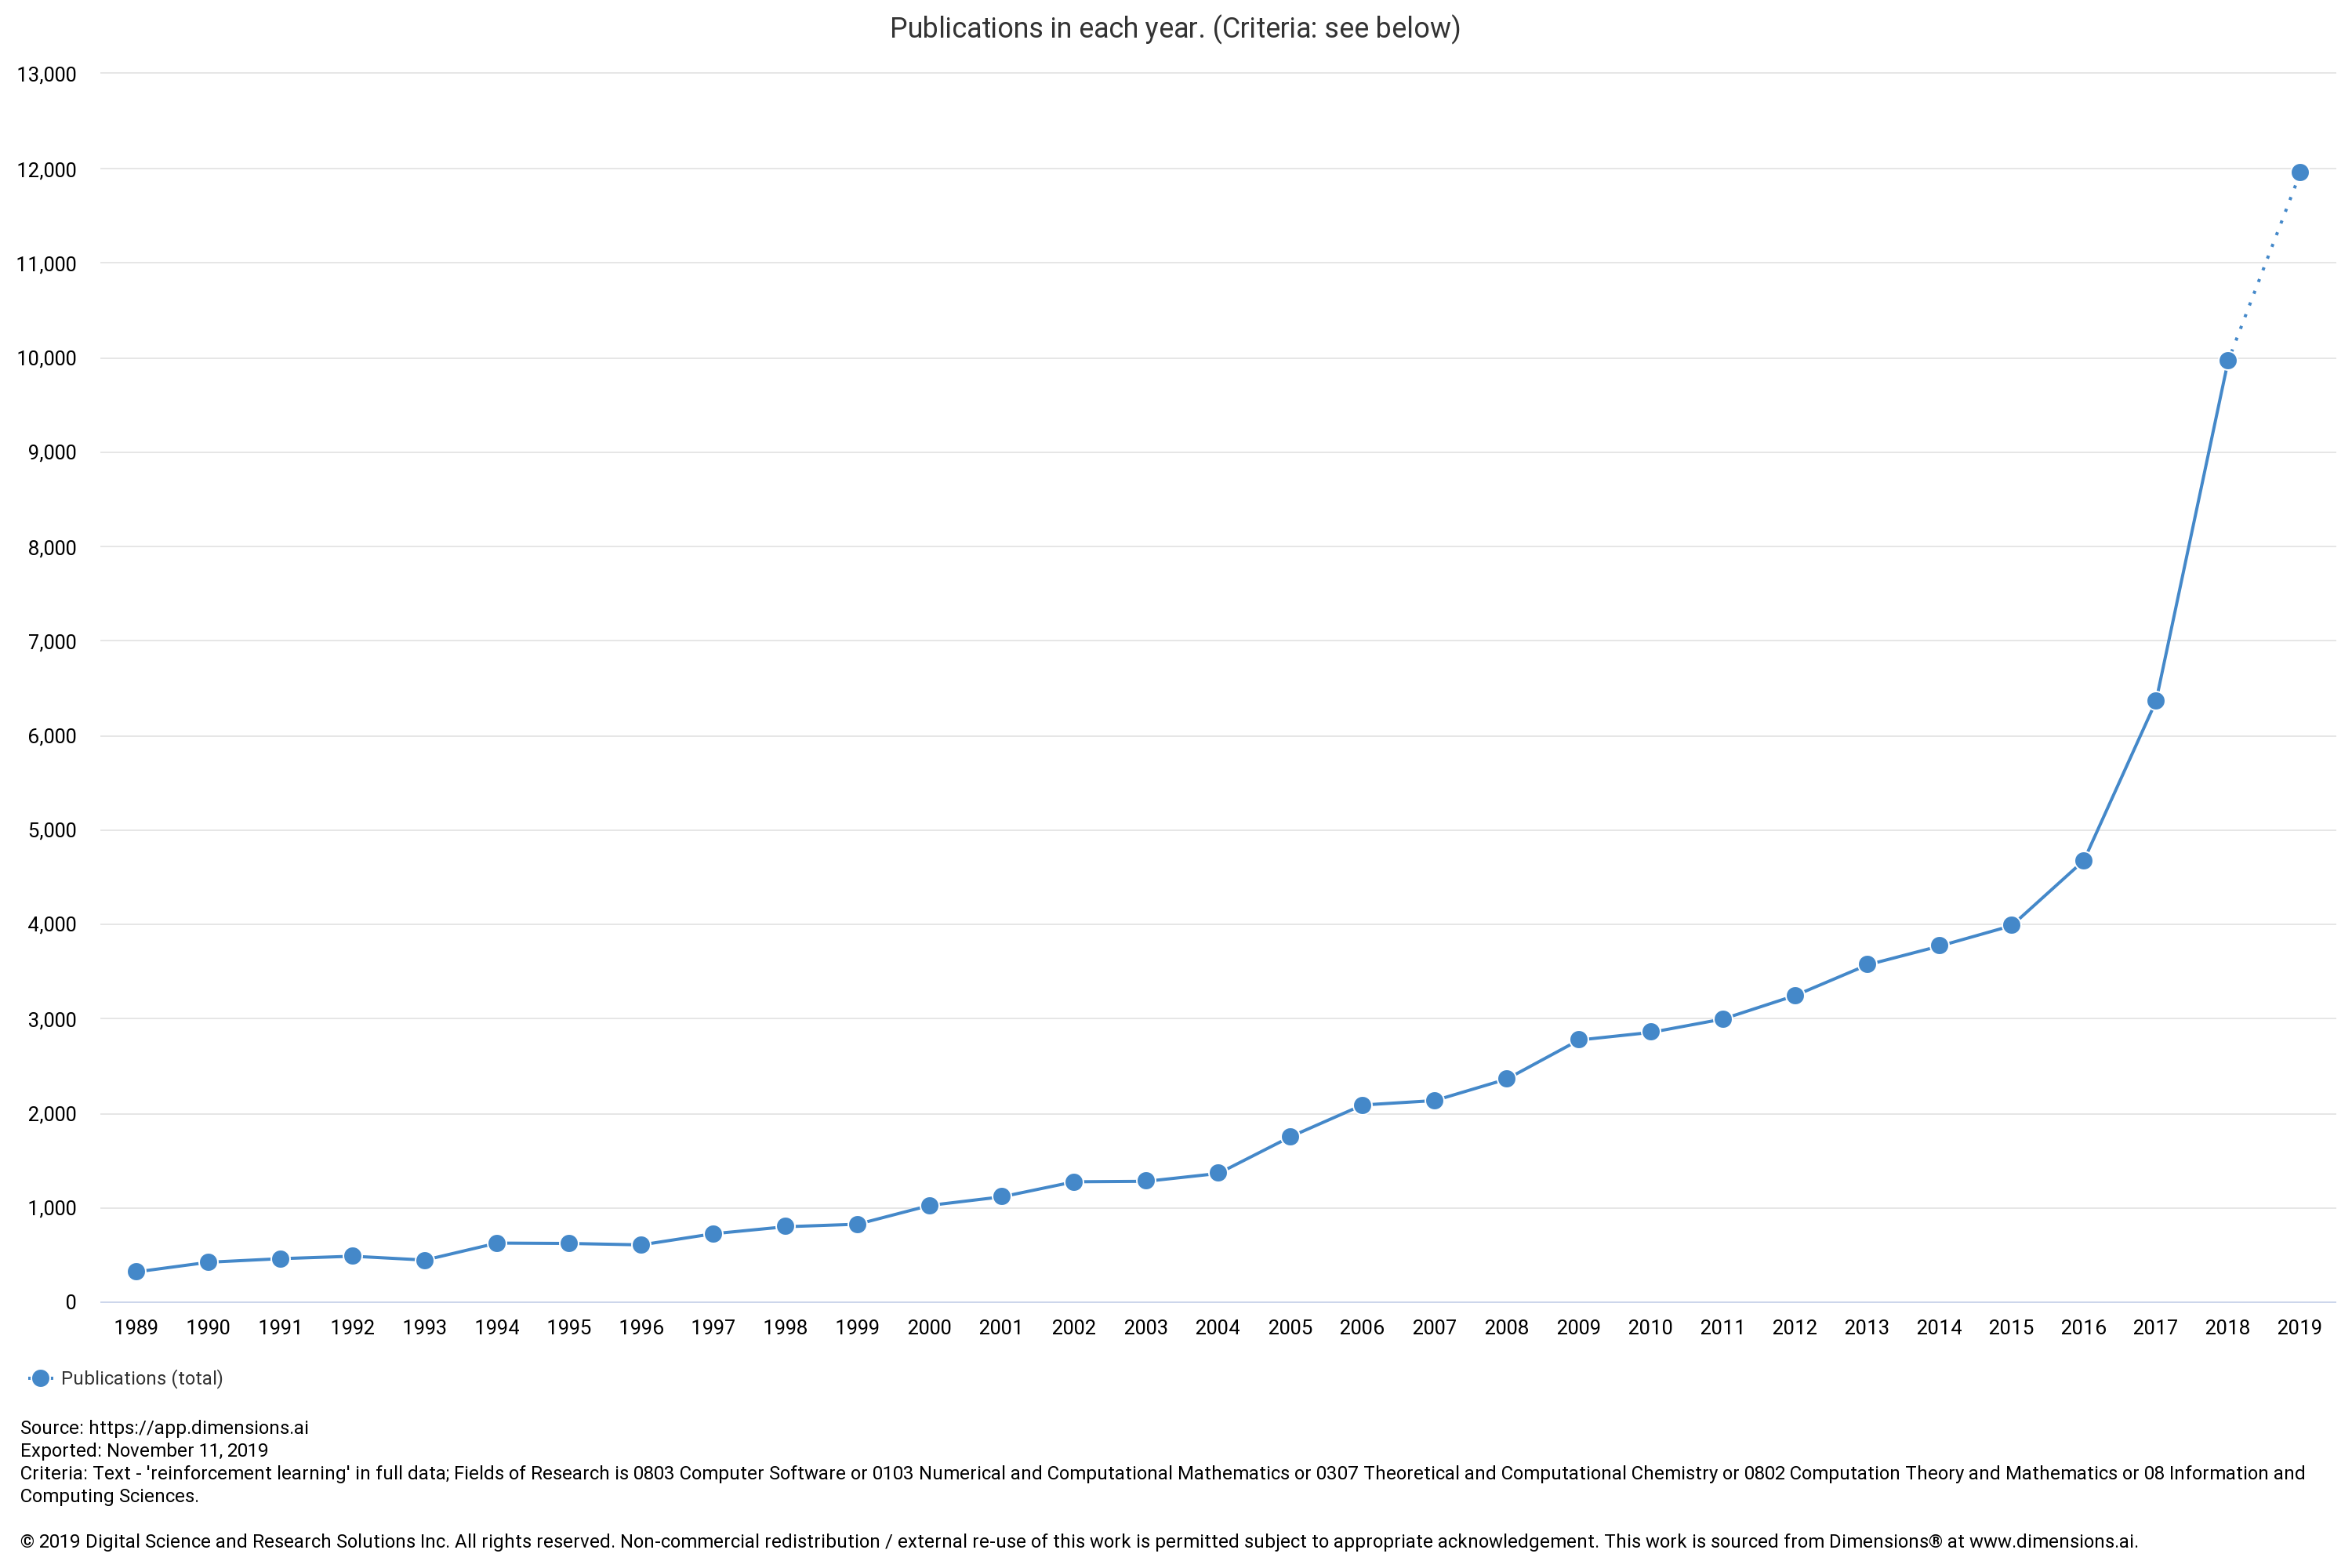
\includegraphics[width=.7 \textwidth]{conteudo/imgs/rl-publications-overview.png}
  \caption[Crescimento do número de publicações sobre RL]{Crescimento do número de publicações sobre \textit{Reinforcement Learning.}}
  \label{rl-publications-overview}
 \end{figure}


Do ponto de vista econômico, são inúmeros os usos de \textit{deep learning} no mercado. Desde ferramentas que melhoram a precisão dos sensores de precipitação por satélite e concentrando-se na redução do viés e dos alarmes falsos \cite{doi:10.1175/JHM-D-15-0075.1}, à agentes que permitem que diferentes dispositivos eletrônicos interpretem dados de multimídia não estruturados e reajam de maneira inteligente aos eventos do usuário e do ambiente \cite{dl-IoT}, o DL tem se tornado cada vez mais presente e essencial para a sociedade. Grandes setores e empresas na área da tecnologia não existiriam sem o uso dessas ferramentas.

Em relação aos impactos sociais do DL podemos mencionar a sua utilização para estimar as características socioeconômicas de regiões de 200 cidades dos Estados Unidos usando 50 milhões de imagens de cenas de rua reunidas com carros do \textit{Google Street View} \cite{Gebru13108}. O DL também teve impactos em diversas áreas da ciência, desde pesquisa em física de partículas \cite{baldi:s:w:2015}, à medicina \cite{nassif:speech-rec:2019}.

É interessante ressaltar que apesar de todos os benefícios oferecidos pela IA, alguns indivíduos notáveis como o famoso físico Stephen Hawking, e o líder da Tesla e da SpaceX Elon Musk, sugerem que a IA pode ser potencialmente muito perigosa. De fato, existem muitos aplicativos de IA que tornam nossa vida cotidiana mais conveniente e eficiente. São os aplicativos de IA que desempenham um papel crítico para garantir a segurança que Musk, Hawking e outros estavam preocupados quando proclamaram sua hesitação sobre a tecnologia. Por exemplo, se a IA for responsável por garantir a operação de nossa rede elétrica, de uma usina nuclear ou outro sistema de alto risco, e a IA for invadida ou tiver seus objetivos desalinhados com os nossos, isso poderá resultar em danos enormes \cite{Marr:AI-Danger}. 

Apesar de todo o medo ao redor dessa nova tecnologia, muitos argumentam que os mesmos são exagerados e que os benefícios oferecidos são muito maiores que os potenciais riscos, desde que sejam gerenciados adequadamente. O crescimento de pesquisas em DRL revelam seu grande potencial e benefícios para a sociedade. Reproduzir e comparar os trabalhos existentes existente e julgar com precisão as melhorias oferecidas por novos métodos é vital para sustentar esse progresso. 



% ----------------------------------------------------------

% ----------------------------------------------------------
% Abordagem proposta 
% ----------------------------------------------------------
% ----------------------------------------------------------
% Abordagem proposta 
% ----------------------------------------------------------
\chapter{Abordagem Proposta}
\label{chap:abordagem}
% ----------------------------------------------------------


No contexto de jogos digitais, treinar um agente para superar os jogadores humanos e otimizar sua pontuação pode nos ensinar como otimizar processos diferentes em uma variedade de subcampos intrigantes \cite{comi:teach:AI:DRL:2018}. Uma solução proposta na literatura, obtendo ótimos resultados, e que tem como objetivo treinar um computador pra aprender e desenvolver estratégias para jogar diferentes jogos, é o \textit{deep reinforcement learning} (DRL). 

No presente trabalho é proposto a implementação de uma inteligência artificial que, utilizando um algoritmo de \textit{deep reinforcement learning}, seja capaz de aprender a jogar diferentes jogos e desenvolver estratégias para maximizar sua pontuação.

Diante das peculiaridades e restrições do problema discutidos em \textbf{\ref{sec:descricao_do_problema}}, a biblioteca \textit{Allegro} foi escolhida como a base para a implementação dos jogos que serão apresentados ao sistema.
O \textit{Allegro} é uma biblioteca multiplataforma destinada principalmente a jogos de vídeo e programação multimídia. A biblioteca fornece rotinas de baixo nível comumente necessárias na programação de jogos, como a criação de janelas, aceitação de entrada do usuário, carregamento de dados, desenho de imagens, reprodução de sons etc \cite{allegro}.

Por fim, para auxiliar a implementação do sistema, será utilizado um \textit{Allegro Learning Enviroment}, uma ferramenta para o desenvolvimento de inteligência artificial em jogos implementados em \textit{Allegro}. Seu objetivo é oferecer uma plataforma que facilite o desenvolvimento de algoritmos de ML para jogos em \textit{Allegro}.



% section contextualização (end)
\section{\textit{Deep Learning}}


 O \textit{deep learning} (DL) é uma área do aprendizado de máquina que propõe que os computadores aprendam com a experiência, se ajustem à novas entradas de dados e compreendam o mundo em termos de hierarquia de conceitos, sendo cada conceito definido por sua relação com conceitos mais simples. 
 Ao reunir conhecimento a partir da experiência, essa abordagem evita a necessidade dos operadores humanos de especificar formalmente todo o conhecimento que o computador precisa. Além disso, a hierarquia de conceitos permite que o computador aprenda conceitos complexos, construindo-os a partir de conceitos mais simples. O \textit{deep learning} apresenta grande poder e flexibilidade a nos permitir o treinamento de computadores para cumprir tarefas específicas ao processar grandes quantidades de dados e reconhecer padrões nesses dados.


 A \textbf{Figura \ref{hierarquia-conceitos-dl}} mostra como um sitema de \textit{deep learning} representa o conceito de imagem de uma pessoa combinando conceitos mais simples, como cantos e contornos, que por sua vez são definidos em termos de arestas. 

 O mapeamento de funções de um conjunto de pixels para uma identidade de objeto é uma tarefa complicada. O algoritmo de \textit{deep learning} resolve essa dificuldade dividindo o mapeamento complicado desejado em séries de mapeamentos simples aninhados, cada um deles descrito por uma camada diferente do modelo. A entrada é apresentada na camada visível,
 em seguida, uma série de camadas ocultas extrai recursos cada vez mais abstratos da imagem. A camada de saída obtém a identidade de objeto abstrata a partir dos conceitos obtidos pelas camadas ocultas.


 \begin{figure}[h]
 \centering
 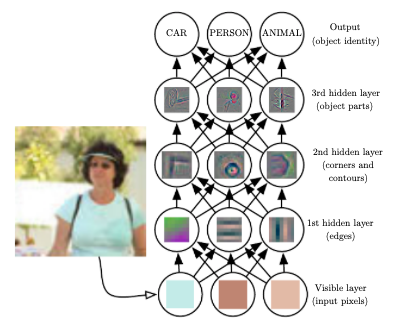
\includegraphics[width=.5 \textwidth]{conteudo/imgs/hierarquia-conceitos-dl.png}
 \caption[Ilustração de um modelo de aprendizado profundo]{Ilustração de um modelo de aprendizado profundo. Cada camada é capaz de identificar dados de complexidade crescente a partir dos pixels pasados para a camada de entrada. Imagem retirada de \cite{Goodfellow-et-al-2016}}
 \label{hierarquia-conceitos-dl}
 \end{figure}
 % \clearpage

 \section{\textit{Reinforcement Learning}} % (fold)
 \label{sec:reinforcement_learning}

 O aprendizado por reforço ou \textit{reinforcement learning} (RL) é uma abordagem computacional para entender e automatizar o aprendizado direcionado a objetivos e a tomada de decisões. O aprendizado por reforço distingue-se de outras abordagens computacionais por sua ênfase na aprendizagem de um agente apartir da interação direta com seu ambiente, sem exigir supervisão exemplar ou modelos completos do ambiente \cite{reinforcement-learning-intro-2018}.

 Em algoritmos de \textit{reinforcement learning}, o agente não é informado sobre quais ações executar, mas, em vez disso, deve descobrir quais ações geram mais recompensa, através de tentativa e erro. Em alguns casos mais interessantes, as ações podem afetar não apenas a recompensa imediata, mas também a próxima situação e, com isso, todas as recompensas subsequentes. Essas duas características - pesquisa por tentativa e erro e recompensa atrasada - são as duas características distintivas mais importantes do aprendizado por reforço.

 % O aprendizado por reforço é diferente do aprendizado supervisionado, o tipo de aprendizado estudado na maioria das pesquisas atuais no campo do aprendizado de máquina. Aprendizado supervisionado é aprender com um conjunto de treinamento de exemplos rotulados fornecidos por um supervisor externo qualificado. O objetivo desse tipo de aprendizado é o sistema extrapolar ou generalizar suas respostas para que ele atue corretamente em situações não presentes no conjunto de treinamento.
 %  % Este é um tipo importante de aprendizado, mas por si só não é adequado para aprender com a interação. Em problemas interativos, muitas vezes é impraticável obter exemplos do comportamento desejado que sejam corretos e representativos de todas as situações nas quais o agente precisa agir. Em um território desconhecido - onde se espera que a aprendizagem seja mais benéfica - um agente deve ser capaz de aprender com sua própria experiência.

 %  O aprendizado por reforço também é diferente do que os pesquisadores de aprendizado de máquina chamam de aprendizado não supervisionado, que geralmente consiste em encontrar estruturas ocultas em coleções de dados não rotulados. Os termos aprendizado supervisionado e aprendizado não supervisionado parecem classificar exaustivamente os paradigmas de aprendizado de máquina, mas não o fazem. Embora se possa ficar tentado a pensar no aprendizado por reforço como um tipo de aprendizado não supervisionado, porque não se baseia em exemplos de comportamento correto, o aprendizado por reforço está tentando maximizar um sinal de recompensa em vez de tentar encontrar uma estrutura oculta. Descobrir a estrutura na experiência de um agente certamente pode ser útil no aprendizado por reforço, mas por si só não aborda o problema do aprendizado por reforço de maximizar um sinal de recompensa. Portanto, o aprendizado por reforço é considerado como um terceiro paradigma de aprendizado de máquina, ao lado de aprendizado supervisionado, aprendizado não supervisionado e talvez outros paradigmas  \cite{reinforcement-learning-intro-2018}.

 Além do agente e do ambiente, é interessante ressaltar outros elementos importantes de um sistema de aprendizado por reforço: a \textbf{política}, o \textbf{sinal de recompensa} e a \textbf{função de valor}.

 A \textbf{política} define a maneira que o agente deve se comportar em um determinado momento. 
 Uma política é basicamente um mapeamento dos estados do ambiente para as ações a serem tomadas quando nesses estados. 
 A política em casos mais simples ter a forma de uma função simples ou uma tabela de pesquisa, enquanto em casos mais complexos pode envolver cálculos mais extensivos. 
 Em geral, as políticas podem ser estocásticas, especificando probabilidades para cada ação.

 Um \textbf{sinal de recompensa} define o objetivo de um problema de aprendizado por reforço. 
 Em cada etapa, o ambiente envia ao agente de aprendizado por reforço um único número que funciona como uma recompensa para o agente. 
 O único objetivo do agente é maximizar a recompensa total que recebe a longo prazo.
 O sinal de recompensa define, portanto, quais são os eventos bons e ruins para o agente. 
 O sinal de recompensa é a base principal para alterar a política - se uma ação selecionada pela política for seguida por uma baixa recompensa, a política poderá ser alterada para selecionar outra ação nessa situação no futuro. 
 Em geral, os sinais de recompensa podem ser funções estocásticas do estado do ambiente e das ações tomadas.

 Enquanto o sinal de recompensa indica o que é bom em um sentido imediato, uma \textbf{função de valor} especifica o que é bom a longo prazo. 
 O valor de um estado representa a quantidade total de recompensa que um agente pode esperar acumular no futuro, a partir desse estado. 
 Enquanto as recompensas determinam a conveniência imediata e intrínseca dos estados ambientais, os valores indicam a conveniência a longo prazo dos estados após levar em conta os estados que provavelmente seguirão e as recompensas disponíveis nesses estados. 
 Por exemplo, um estado sempre pode gerar uma recompensa imediata baixa, mas ainda tem um valor alto porque é seguido regularmente por outros estados que produzem recompensas altas. Ou o contrário poderia ser verdade. 

 A \textbf{Figura \ref{rl-diagram}} mostra um diagrama de aprendizagem por reforço relacionando o agente de aprendizado com o ambiente no qual ele é inserido.
 O ambiente representa o mundo pelo qual o agente se move. O ambiente nada mais é do que um sistema que toma o estado atual e a ação do agente como entrada e retorna como saída a recompensa do agente e seu próximo estado. 

 Ambientes podem ser modelados como funções que transformam uma ação executada no estado atual, no próximo estado e uma recompensa. Já os agentes podem ser modelados como funções que transformam o novo estado e recompensam na próxima ação. 
 Podemos conhecer a função do agente, mas não podemos conhecer a função do ambiente. É uma caixa preta onde só vemos as entradas e saídas. 
 % É como o relacionamento da maioria das pessoas com a tecnologia: sabemos o que faz, mas não sabemos como funciona. 
 O aprendizado por reforço representa a tentativa de um agente de aproximar a função do ambiente, para que possamos enviar ações para o ambiente de caixa preta que maximize as recompensas que ele distribui \cite{beg-guide-rl}.

 \begin{figure}[h]
  \centering
  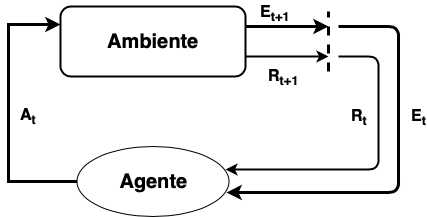
\includegraphics[width=.6 \textwidth]{conteudo/imgs/rl-diagram.png}
  \caption[Diagrama de aprendizagem por reforço]{Diagrama de aprendizagem por reforço. No \textit{loop} de \textit{feedback} acima, os subscritos indicam as etapas de tempo $t$ e $t + 1$, cada uma das quais se refere a estados diferentes: o estado no momento $t$ e o estado no momento $t + 1$. 
 % Diferente de outras formas de aprendizado de máquina - como aprendizado supervisionado e não supervisionado - o aprendizado por reforço só pode ser pensado sequencialmente em termos de pares de ação de estado que ocorrem um após o outro.
  A ação $A_t$ de um agente é determinada por sua \textbf{política}, que por sua vez é uma função que depende do estado atual do sistema $E_t$. A política de um agente tem como objetivo maximizar a \textbf{função de valor} que é calculada utilizando o \textbf{sinal de recompensa} $R_t$. O ambiente se comporta como um sistema caixa preta que transforma uma ação executada no estado atual $A_t$, no próximo estado $E_{t+1}$ e uma recompensa $R_{t+1}$
  }
  \label{rl-diagram}
 \end{figure}

 As escolhas de ação são feitas com base em julgamentos de valor.
 Buscamos ações que gerem estados de maior valor, e não de maior recompensa, porque essas ações obtêm a maior quantidade de recompensa a longo prazo. 
 % Infelizmente, é muito mais difícil determinar valores do que determinar recompensas. 
 As recompensas são basicamente dadas diretamente pelo ambiente, mas os valores devem ser estimados e re-estimados a partir das sequências de observações que um agente faz ao longo de toda a sua vida útil.


 O \textit{deep reinforcement learning} (DRL) é uma abordagem do \textit{deep learning} que, em contraste a abordagens mais tradicionais como o aprendizado supervisionado e não supervisionado, utiliza as técnicas de aprendizagem por reforço para treinar o agente. Essa abordagem consiste em fornecer ao sistema parâmetros relacionados ao seu estado e uma recompensa positiva ou negativa com base em suas ações. Nenhuma regra sobre o jogo é dada e, inicialmente, o agente não tem nenhuma informação sobre o que precisa fazer. O objetivo do sistema é descobrir e elaborar uma estratégia para maximizar sua pontuação - ou recompensa.



\section{Aplicação de DRL em um \textit{Allegro Learning Enviroment}} % (fold)
 \label{sec:allegro_learning_enviroment}

 O \textit{Arcade Learning Enviroment} é uma ferramenta de software que oferece uma interface para interagir com ambientes de jogos Atari 2600 emulados. Seu objetivo é oferecer uma plataforma que facilite o desenvolvimento de agentes de aprendizado para aprender a jogar jogos Atari. Essa ferramenta também fornece uma camada de manipulação de jogos que
 transforma cada jogo em um problema padrão de aprendizado por reforço, identificando a pontuação acumulada e se o jogo terminou. \cite{arcade-learning-enviroment}

 Inspirado na plataforma descrita acima, este trabalho visa a utilização de um \textit{Allegro Learning Enviroment}, que funcionaria de forma semelhante ao \textit{Arcade Learning Enviroment}, com a distinção de que o primeiro seria uma plataforma voltada para jogos implementados em \textit{Allegro}. O \textit{Allegro Learning Enviroment} (ALE) terá como base a ferramenta implementada por \cite{silva:amb-jd-allegro}, que oferece um ambiente facilitador ao estudo de soluções de IA aplicada em jogos. Essa ferramenta fornece funcionalidades como a exportação dos comandos básicos de um jogo, que precisam ser passados para o agente para que o mesmo tenha conhecimento dos limites físicos do ambiente no qual está inserido. Isso permite que o pesquisador não fique limitado a um jogo existente, mas possa usar qualquer jogo que ele tenha acesso ao código fonte e feito em \textit{Allegro}.

 Para o treinamento do agente, serão utilizados capturas da tela em cada estado do jogo, obtidas pelo ALE. A partir dessas imagens serão extraídas  as informações do estado atual do jogo (posição do jogador, obstáculos, etc), de forma a determinar qual a melhor ação do agente para a situação na qual ele se encontra. A utilização de capturas de tela como entradas para o agente permite que a IA seja treinada para situações em que hajam obstáculos gerados de forma aleatória. A partir dessas imagens, o agente deverá ser capaz de identificar tais obstáculos, sua localização e a melhor maneira de lidar com os mesmos.

 Em relação aos jogos nos quais o agente será treinado, a proposta é de se utilizar diferentes jogos de diferentes complexidades para avaliar o potencial do sistema. Os jogos serão obtidos de fontes de código aberto disponíveis \textit{online} ou, caso seja necessário, serão implementados com os requisitos necessário para o projeto.



 

 % [TODO]


 % \section{Modelagem matemática} % (fold)
 % \label{sec:modelagem_matemática}
 
 % section modelagem_matemática (end)





% ----------------------------------------------------------


% % ----------------------------------------------------------
% % Introdução (exemplo de capítulo sem numeração, mas presente no Sumário)
% % ----------------------------------------------------------
% \chapter{Introdução}
% % ----------------------------------------------------------

% Este documento e seu código-fonte são exemplos de referência de uso da classe
% \textsf{abntex2} e do pacote \textsf{abntex2cite}. O documento 
% exemplifica a elaboração de trabalho acadêmico (tese, dissertação e outros do
% gênero) produzido conforme a ABNT NBR 14724:2011 \emph{Informação e documentação
% - Trabalhos acadêmicos - Apresentação}.

% A expressão ``Modelo Canônico'' é utilizada para indicar que \abnTeX\ não é
% modelo específico de nenhuma universidade ou instituição, mas que implementa tão
% somente os requisitos das normas da ABNT. Uma lista completa das normas
% observadas pelo \abnTeX\ é apresentada em \citeonline{abntex2classe}.

% Sinta-se convidado a participar do projeto \abnTeX! Acesse o site do projeto em
% \url{http://www.abntex.net.br/}. Também fique livre para conhecer,
% estudar, alterar e redistribuir o trabalho do \abnTeX, desde que os arquivos
% modificados tenham seus nomes alterados e que os créditos sejam dados aos
% autores originais, nos termos da ``The \LaTeX\ Project Public
% License''\footnote{\url{http://www.latex-project.org/lppl.txt}}.

% Encorajamos que sejam realizadas customizações específicas deste exemplo para
% universidades e outras instituições --- como capas, folha de aprovação, etc.
% Porém, recomendamos que ao invés de se alterar diretamente os arquivos do
% \abnTeX, distribua-se arquivos com as respectivas customizações.
% Isso permite que futuras versões do \abnTeX~não se tornem automaticamente
% incompatíveis com as customizações promovidas. Consulte
% \citeonline{abntex2-wiki-como-customizar} para mais informações.

% Este documento deve ser utilizado como complemento dos manuais do \abnTeX\ 
% \cite{abntex2classe,abntex2cite,abntex2cite-alf} e da classe \textsf{memoir}
% \cite{memoir}. 

% Esperamos, sinceramente, que o \abnTeX\ aprimore a qualidade do trabalho que
% você produzirá, de modo que o principal esforço seja concentrado no principal:
% na contribuição científica.

% Equipe \abnTeX 

% Lauro César Araujo

% % ----------------------------------------------------------
% % PARTE
% % ----------------------------------------------------------
% \part{Preparação da pesquisa}
% % ----------------------------------------------------------

% % ---
% % Capitulo com exemplos de comandos inseridos de arquivo externo 
% % ---
% \include{abntex2-modelo-include-comandos}
% % ---

% \chapter{Conteúdos específicos do modelo de trabalho acadêmico}\label{cap_trabalho_academico}

% \section{Quadros}

% Este modelo vem com o ambiente \texttt{quadro} e impressão de Lista de quadros 
% configurados por padrão. Verifique um exemplo de utilização:

% \begin{quadro}[htb]
% \caption{\label{quadro_exemplo}Exemplo de quadro}
% \begin{tabular}{|c|c|c|c|}
% 	\hline
% 	\textbf{Pessoa} & \textbf{Idade} & \textbf{Peso} & \textbf{Altura} \\ \hline
% 	Marcos & 26    & 68   & 178    \\ \hline
% 	Ivone  & 22    & 57   & 162    \\ \hline
% 	...    & ...   & ...  & ...    \\ \hline
% 	Sueli  & 40    & 65   & 153    \\ \hline
% \end{tabular}
% \fonte{Autor.}
% \end{quadro}

% Este parágrafo apresenta como referenciar o quadro no texto, requisito
% obrigatório da ABNT.
% Primeira opção, utilizando \texttt{autoref}: Ver o \autoref{quadro_exemplo}. 
% Segunda opção, utilizando  \texttt{ref}: Ver o Quadro \ref{quadro_exemplo}.

% % ----------------------------------------------------------
% % PARTE
% % ----------------------------------------------------------
% \part{Referenciais teóricos}
% % ----------------------------------------------------------

% % ---
% % Capitulo de revisão de literatura
% % ---
% \chapter{Lorem ipsum dolor sit amet}
% % ---

% % ---
% \section{Aliquam vestibulum fringilla lorem}
% % ---

% \lipsum[1]

% \lipsum[2-3]

% % ----------------------------------------------------------
% % PARTE
% % ----------------------------------------------------------
% \part{Resultados}
% % ----------------------------------------------------------

% % ---
% % primeiro capitulo de Resultados
% % ---
% \chapter{Lectus lobortis condimentum}
% % ---

% % ---
% \section{Vestibulum ante ipsum primis in faucibus orci luctus et ultrices
% posuere cubilia Curae}
% % ---

% \lipsum[21-22]

% % ---
% % segundo capitulo de Resultados
% % ---
% \chapter{Nam sed tellus sit amet lectus urna ullamcorper tristique interdum
% elementum}
% % ---

% % ---
% \section{Pellentesque sit amet pede ac sem eleifend consectetuer}
% % ---

% \lipsum[24]

% % ----------------------------------------------------------
% % Finaliza a parte no bookmark do PDF
% % para que se inicie o bookmark na raiz
% % e adiciona espaço de parte no Sumário
% % ----------------------------------------------------------
% \phantompart

% % ---
% % Conclusão
% % ---
% \chapter{Conclusão}
% % ---

% \lipsum[31-33]

% ----------------------------------------------------------
% Referências bibliográficas
% ----------------------------------------------------------
\bibliography{conteudo/postextual/referencias}
% ----------------------------------------------------------
% ELEMENTOS PÓS-TEXTUAIS
% ----------------------------------------------------------
%\postextual
% ----------------------------------------------------------

% ----------------------------------------------------------
% Referências bibliográficas
% ----------------------------------------------------------
\bibliography{conteudo/postextual/referencias}

% ----------------------------------------------------------
% Glossário
% ----------------------------------------------------------
%
% Consulte o manual da classe abntex2 para orientações sobre o glossário.
%
%\glossary

% ----------------------------------------------------------
% Apêndices
% ----------------------------------------------------------
%% ---
% Inicia os apêndices
% ---
\begin{apendicesenv}

% Imprime uma página indicando o início dos apêndices
\partapendices

% ----------------------------------------------------------
\chapter{Quisque libero justo}
% ----------------------------------------------------------

\lipsum[50]

% ----------------------------------------------------------
\chapter{Nullam elementum urna vel imperdiet sodales elit ipsum pharetra ligula
ac pretium ante justo a nulla curabitur tristique arcu eu metus}
% ----------------------------------------------------------
\lipsum[55-57]

\end{apendicesenv}
% ---


% ----------------------------------------------------------
% Anexos
% ----------------------------------------------------------
%% ---
% Inicia os anexos
% ---
\begin{anexosenv}

% Imprime uma página indicando o início dos anexos
\partanexos

% ---
\chapter{Morbi ultrices rutrum lorem.}
% ---
\lipsum[30]

% ---
\chapter{Cras non urna sed feugiat cum sociis natoque penatibus et magnis dis
parturient montes nascetur ridiculus mus}
% ---

\lipsum[31]

% ---
\chapter{Fusce facilisis lacinia dui}
% ---

\lipsum[32]

\end{anexosenv}


%---------------------------------------------------------------------
% INDICE REMISSIVO
%---------------------------------------------------------------------
\phantompart
\printindex
%---------------------------------------------------------------------


\end{document}
